\documentclass{book}
\usepackage[utf8]{inputenc}
\usepackage[spanish]{babel}
\usepackage{graphicx}% Paquete para agregar gráficos
\usepackage{multicol} % Paquete para agregar varias columnas
\usepackage{listings} % Paquete para agregar código
\usepackage{hyperref} % Paquete para agregar hiperlinks (NAVEGACIÓN A TRAVÉS DEL DOCUMENTO), como la imagen.
\usepackage{enumerate} % enumerados
\usepackage{verbatim} % comentarios
\usepackage{amsmath}
\usepackage{amssymb} % Para alfabetos matemáticos

\usepackage{biblatex}
\usepackage{csquotes}
\addbibresource{referencias.bib}

\title{Geoestadística}
\author{Laydi Viviana Bautista}
\date{Mayo 2019}


\begin{document}


%%%%%%%%%%%%%%%%%%%%%%%%%%%%%%%%%%%%%%%5
%%%%%%%%%%%%%%%%%%%%%%%%%%%%%%%%%%%%%%%%
%Ramas de la Estadistica Espacial: Geoestadistica, Lattices y Patrones espaciales
%\section{Dependencia Espacial}

La dependencia espacial hace referencia a la estructura de correlación de las variables aleatorias del proceso
${Z(s) : s \in D \subset R^d }$. Cuando hay dependencia espacial los sitios
cercanos tienen valores más similares que los distantes. Por el contrario la ausencia de correlación espacial se refleja en el hecho de que la distancia entre los sitios no tiene influencia
en la relación de sus valores. \cite{giraldo}

\subsection{Test de Moran}

Este test es especialmente usado en datos de áreas. Sean $Z(s_1 ), · · · , Z(s_n)$, las variables medidas en las $n$ áreas. La noción de autocorrelación espacial de estas variables está asociada con la idea de que valores observados en áreas geográficas adyacentes serán más similares que los esperados bajo el supuesto de independencia espacial. El ı́ndice de autocorrelación de Moran considerando la información de los vecinos más cercanos es definida
como:

$$ I = \frac{n}{\Sigma}$$

Valores positivos (entro 0 y 1) indican autocorrelación directa (similitud entre valores cercanos) y valores negativos (entre -1 y 0) indican autocorrelación inversa (disimilitud entre las áreas cercanas). Valores del coeficiente cercanos a cero apoyan la hipótesis de aleatoriedad espacial.

Para el cálculo del índice de Moran es necesario definir la proximidad entre las áreas. Lo anterior se lleva a cabo por medio del cálculo de una matriz de proximidad espacial. 








%\section{Inferencia Estadística}

Mucho métodos estadísticos están basados en el supuesto de que las variables aleatorias involucradas en la muestra son independientes. La violación de dicho supuesto tiene consecuencias en todos los procesos inferenciales. 

%Tarea: al optemer la meseta compararlo con el valor de la varianza de la variable


%%%%%%%%%%%%%%%%%%%%%%%%%%%%%%%%%%%%%%


\chapter{Marco Teórico}



\section{Estadística Espacial}

La Estadística espacial es la reunión de un conjunto de metodologías apropiadas para el
análisis de datos que corresponden a la medición de variables aleatorias en diversos sitios, ya sean estps puntos del espacio o agregaciones espaciales de una región. 

De manera más formal se puede decir que la estadística espacial trata con el análisis de 
realizaciones de un proceso estocástico   $${ Z ( s ) : s \in D }$$  donde $S$ representa un ubicación en el espacio euclidiano $R^d$ d-dimensional y varía sobre un conjunto de índices $D \subset R^d$.  $Z(s)$ es una variable aleatoria en
la ubicación $s$ y el conjunto índice $D$ puede ser continuo, discreto o aleatorio.\cite{giraldo}


Esta ramificación de la Estadística surge, entre otras cosas, de la necesidad de generar métodos de análisi que se ajusten a las características de los datos espaciales, los cuales no cumplen, en particular, con el supuesto de independencia propuesto en el análisis clásico. La correlación entre los datos espaciales es "proporcional" a la distancia que separa a las ubicaciones en donde se realizaron las mediciones; esta premisa se puede soportar en una de las leyes de Tobler que dice "Todo esta relacionado con todo lo demás, pero cosas cercanas están más relacionadas que cosas distantes"\cite{notas_clase2}


La estadística espacial se subdivide en tres grandes áreas: La geoestadistica, lattices y patrones espaciales. La pertinencia de cada una
de ellas está asociada a las características del conjunto $D$ de índices del proceso estocástico
de interés. 

  


\section{Geoestadística}


Las ubicaciones $s$ provienen de un conjunto $D$ continuo  y son seleccionadas
a juicio del investigador ($D$ fijo), es decir que el investigador puede hacer selección de puntos del espacio a conveniencia o seleccionar los sitios bajo algún esquema de muestro probabilístico. Algunos ejemplos  son: Niveles de un contaminante en diferentes sitios de una
parcela, contenidos auríferos de una mina, valores de precipitación en Colombia medida en
las diferentes estaciones meteorológicas en un mes dado o los niveles piezométricos de un
acuífero. En los ejemplos anteriores es claro que hay continuidad espacial, puesto que en
cualquier sitio de la parcela, de la mina, de Colombia o del acuífero pueden ser medias las
correspondientes variables.

Es importante resaltar que en geoestadística el propósito esencial es la interpolación y si no hay continuidad espacial pueden hacerse predicciones carentes de sentido. \cite{giraldo}

Cuando el objetivo es hacer predicción, se realiza dos etapas: análisis estructural (describir la correlación en puntos del espacio) y la segunda etapa es la predicción en sitios no muestrarios por medio de Kriging (proceso que calcula el promedio ponderado de las observaciones muestrales). Los pesos asignados a los valores muestrales son apropiadamente determinados por la estructura espacial de correlación establecida en la primera etapa y por la configuración de muestro (Petitgas, 1996 citado por \cite{giraldo})

La primera etapa en el desarrollo de un análisis geoestadístico es la determinación de la dependencia espacial entre los datos medidos de una variable. Esta fase es también conocida como análisis estructural. \cite{giraldo}



\chapter{Introducción}

\section{Introducción}

Se presentan los registros de la temperatura media terrestre de Croacia referente al --------día 13 de marzo de 2008------, los cuales fueron sometidos a un tratamiento estadístico mediante pruebas de
normalidad, tendencia y anisotropía, que fueron evaluadas previamente para finalmente realizar el
ajuste del variograma. El procedimiento se llevó a cabo en el software R.


\section{Objetivo}

Realizar el ajuste del variograma a través del modelamiento de la variación espacial para los registros de la temperatura media terrestre diaria de Croacia.

\subsection{Objetivos Específicos}

\begin{itemize}
    \item Elaborar un análisis exploratorio mediante pruebas (normalidad, tendencia y anisotropía),
observando y valorando el comportamiento de los registros para la respectiva elección del
modelo.

\end{itemize}

\section{Justificación}

El cambio climático se ha convertido en una gran preocupación que afecta a todo el globo debido a las consecuencias que traerá a generaciones futuras. Este, implica el incremento de condiciones extremas
que se traducen en sequías, olas de calor, inundaciones, entre otros.  (Stott et al. \cite{stott_ea})

La  correcta  evaluación  de  los  distintos  elementos  del  tiempo  atmosférico  y  del  clima  requiere cada día mayor precisión. Además del propio interés científico, el contar con información meteorológica depurada y representada espacialmente, teniendo en cuenta las peculiaridades morfológicas de la región en la que incide, interviene positivamente en numerosas tareas de planificación hidrológica, agrícola, urbanística, etc. dicha  información  procede  en  gran  medida  de  redes  meteorológicas  de  superficie,  de  densidad  frecuentementebaja  y  ubicación  preferente  en  fondos  de  valle,  lo  que  obliga  a  emplear  algoritmos  de  estimación  espacial  para acercarse a la realidad meteorológica en aquellas zonas no muestreadas. (Hernan, 2000 \cite{hernan_ea})

\\
El   objetivo   del   presente   estudio para nuestro caso, la implementación del tratamiento estadístico
(análisis exploratorio) y técnicas geoestadísticas, permiten estimar el comportamiento de la
temperatura a partir de 158 registros de estaciones meteorológicas localizadas en la superficie de Croacia

\section{Estado del arte}

Según ( Socha, s.f)  \cite{temp_boyaca}  las  técnicas  de  predicción  geoestadisticas  proveen  la  correcta  manera  de analizar  fenómenos  naturales  que  ocurren  en  una  determinada  extensión  geográfica  logrando predecir  información  de  áreas  en  las  que  no  se  tiene    mediciones  y  de  esta  manera  extender  la cobertura  del  estudio  para  toda  el  área  de  interés, en el estudio realizado por (Sanchéz, 2011) \cite{sanchez_ea} estudia la estimación de la temperatura media anual  en  la  región  sureste  del  estado  de  Coahuila  a  través  de  21  estaciones  climatológicas  dependientes del Servicio Meteorológico Nacional, seleccionando  para la interpolación Kriging  el  modelo  Gaussiano, 
( Socha, s.f) \cite{temp_boyaca}  por su parte mediante el  ``análisis tendencial de la variación climática `Temperatura y precipitación' espacio-temporal del departamento de Boyacá''  realizó el análisis a series  de  tiempo  de  29 estaciones meteorológicas del Departamento de Boyacá, con registros que datan de 1997 y 2001  generó los Mapas de tendencia de la variable de Temperatura y teniendo en cuenta que la muestra se clasificó como paramétrica se utilizó el Método de Kriging Disyuntivo ya que es el único método que maneja el software (ArcGis) para los datos con distribución paramétrica. Este método requiere de hacer fuertes premisas asumiendo que todos los pares de datos vienen en una distribución normal bivariada. Para la generación de los Mapas de tendencia de la variable de Precipitación y teniendo en cuenta que la muestra se clasificó como No Paramétrica se utilizó el
Método de Kriging Ordinario ya que es un buen método para analizar datos no paramétrico. 

En este caso, el análisis de la correlación espacial nos confirma la relación e influencia entre las variables precipitación y temperatura. El resultado del análisis realizado a las 29 estaciones meteorológicas en el Departamento de Boyacá se evidencian de forma espacial mediante los mapas de tendencia los cuales nos permiten ver de forma clara el comportamiento de la variable tanto espacialmente como temporalmente ya que al hacer la comparación entre los dos años de la misma variable se pueden
evidenciar claramente los cambios presentes o no en los dos periodos de tiempo analizados.

\begin{figure}
    \centering
    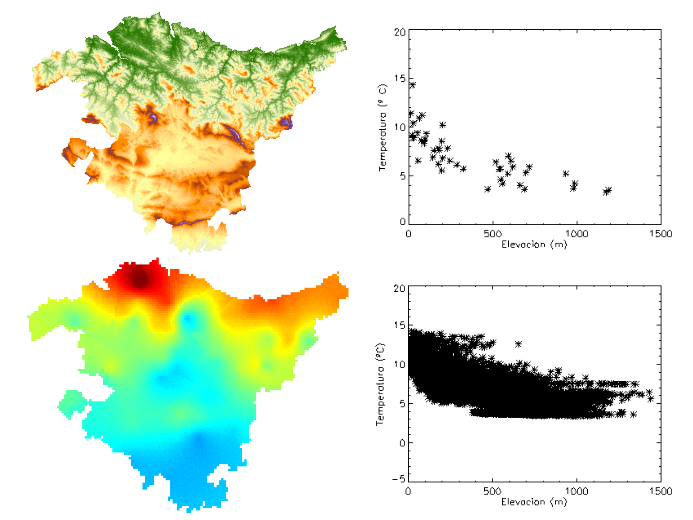
\includegraphics[scale=0.4]{proyectos/proyecto_geoestadistica_croacia/images/ea_hernan_mp.png}
    \caption{ a) Modelo digital de elevaciones de la C.A. del País Vasco; b) gráfica de dispersión elevación-temperatura muestral; c) mapa de temperatura estimada por KO (W(u) = 8); d) gráfica de dispersión elevación-temperatura estimada}
    \label{ea_hernan}
\end{figure}
\\
 (Hunter & Meentemeyer, 2005) \cite{ea_hunter}  en el caso de estudio ``Mapeo Climatológico asistido de la Precipitación y Temperatura Diaria." presenta el método PRISM que permite mapear las condiciones climáticas diarias que integra una red de observaciones de punto de estación base con mapas de clima de promedio a largo plazo, este método supone que la elevación es uno de los factores más importantes que controlan los patrones de temperatura y humedad del paisaje, y utiliza la regresión lineal para estimar la variabilidad climática dentro de las orientaciones topográficas locales, y el kriging ordinario permitiendo interpolar las observaciones puntuales de la red de estaciones base meteorológicas, para el caso de estudio utilizo  la base de datos del Centro Nacional de Datos Climáticos (NCDC) de la Administración Nacional Oceánica y Atmosférica (NOAA) que contiene 24 años de parámetros climáticos diarios (1980-2003) en 779 ubicaciones de puntos en el condado de California, teniendo como resultado para temperaturas máximas y mínimas modelos que predijeron 92\% y 89\% de la variación en los valores diarios observados, respectivamente.


\begin{figure}
    \centering
    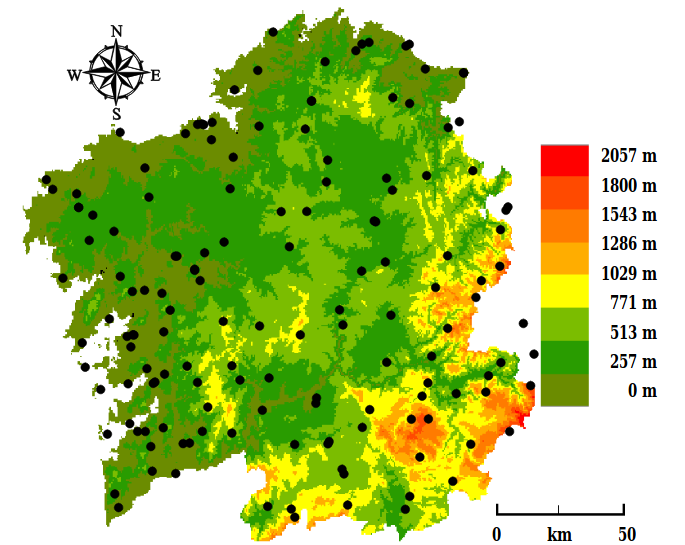
\includegraphics[scale=0.4]{proyectos/proyecto_geoestadistica_croacia/images/ea_galicia.png}
    \caption{Modelo de elevación digital (MDE) de Galicia y localización geográfica de las 151 estaciones meteorológicas que proporcionaron datos continuos en el año 2011}
    \label{ea_galicia}
\end{figure}


\begin{figure}
    \centering
    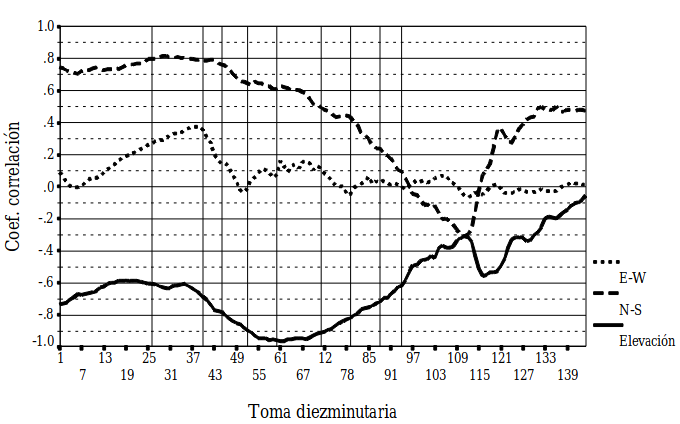
\includegraphics[scale=0.4]{proyectos/proyecto_geoestadistica_croacia/images/ea_henao_i.png}
    \caption{Correlación de la temperatura con la elevación y las direcciones N-S y E-W durante el día 24/04/99, y tomas diezminutarias seleccionadas}
    \label{ea_hernan_i}
\end{figure}

\\
Por otro lado, (Hernan, 2000) \cite{hernan_ea} el caso de estudio ``Estimación Espacial de la Temperatura del Aire mediante Kriging con Deriva Externa''  se realizó la estimación  de  la  temperatura  del  aire  introduciendo  la  elevación del  terreno  como  información  secundaria, (ver figura \ref{ea_hernan_i}) según los resultados se aplico KO, KT y KDE a las tomas diezminutarias seleccionadas, repitiendo el proceso para  dos  vecindarios  de  diferente  tamaño,  compuestos  por  8  y  16  estaciones, y realizando la comparación de los métodos mediante  validación  cruzada, obtuvo que  los  métodos  univariados  ofrecen mejores  resultados  que  el  KDE  siempre  que  el  coeficiente  de  correlación  entre  la  elevación  y  la temperatura sea inferior a 0.9.  Sin  embargo,  esta conclusión puede  llevar  a  engaño  a  la  hora  de  cartografiar  la temperatura, ya que los mapas (ver figura \ref{ea_hernan}) producidos mediante KO o KT no son satisfactorios en las zonas de montaña, donde la densidad de las estaciones no es suficiente para reproducir los complejos patrones espaciales que se dan entre ambas variables, es entonces donde  el kriging  con  deriva  externa  KDE, estimador  que  incorpora  datos secundarios exhaustivamente muestreados para la caracterización de la tendencia espacial del atributo primario, se presenta como mejor método ya que la  inclusión  de  la  elevación  del  terreno  mejora  significativamente  la  representación  espacial de  la  temperatura  sensor izada, al  ser  un  atributo  secundario  altamente muestreado,   introducido   en   forma   de   MDE,   complementa   las   lagunas   muestrales   de   la   red termométrica.


\begin{figure}
    \centering
    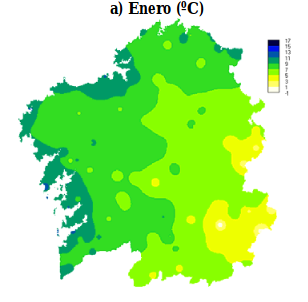
\includegraphics[scale=0.6]{proyectos/proyecto_geoestadistica_croacia/images/ea_galicia_di.png}
    \caption{Interpolación de la temperatura en Galicia mediante el método de distancias inversas para enero en el año de 2011}
    \label{ea_galicia_di}
\end{figure}


\begin{figure}
    \centering
    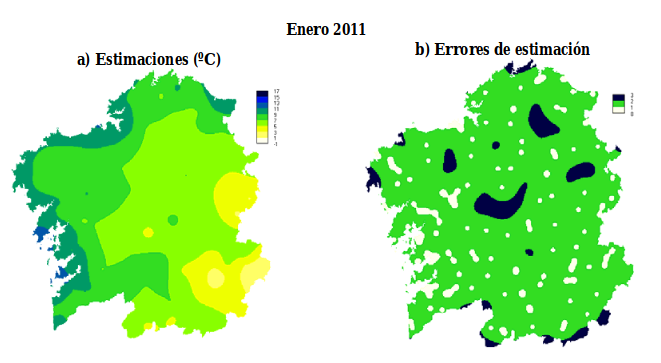
\includegraphics[scale=0.6]{proyectos/proyecto_geoestadistica_croacia/images/ea_galicia_ko.png}
    \caption{Interpolación de la temperatura en Galicia mediante el método de krigeado ordinario para enero con sus respectivos mapas de errores}
    \label{ea_galicia_ko}
\end{figure}


\begin{figure}
    \centering
    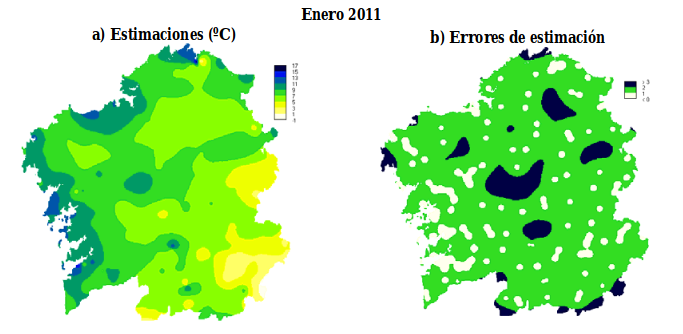
\includegraphics[scale=0.6]{proyectos/proyecto_geoestadistica_croacia/images/ea_galicia_coko.png}
    \caption{Interpolación  de  la  temperatura  en  Galicia  mediante  el  método  del  co-krigeado  ordinario  para  enero de  2011  con  sus  respectivos  mapas  de  errores}
    \label{ea_galicia_coko}
\end{figure}

\begin{figure}
    \centering
    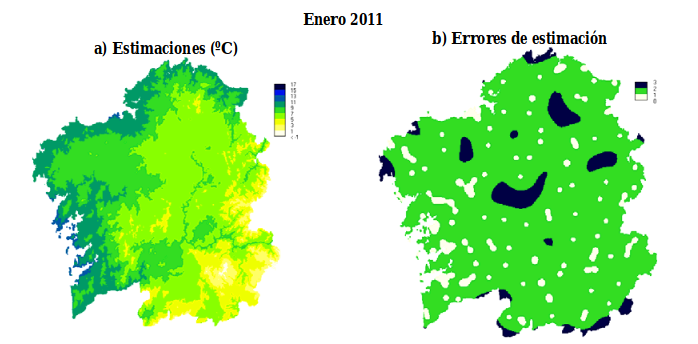
\includegraphics[scale=0.6]{proyectos/proyecto_geoestadistica_croacia/images/ea_galicia_kde.png}
    \caption{ Interpolación de la temperatura en Galicia mediante el método del krigeado con  deriva  externa  para  enero de  2011  con  sus  respectivos  mapas  de  errores}
    \label{ea_galicia_kde}
\end{figure}

Para le caso de (Machado, 2017 \cite{galicia_ea}) en ``Variabilidad Espacial de la Temperatura  en Galicia a Escala Mensual'' (ver figura \ref{ea_galicia}) concluyeron que  la cartografía de la temperatura por el método de las distancias inversas (ver figura \ref{ea_galicia_di}) puso de manifiesto que dicho método puede ser adecuado para una rápida caracterización de la temperatura.  Sin  embargo,  los  mapas  obtenidos  mediante  este  método,  en  general  presentan  un  aspecto  caracterizado  por  la  presencia  de  discontinuidades  o  anomalías  espaciales, con respecto a los  semivariogramas  ajustados  a  las  series  de  temperatura  media  mensual  presentaron meseta bien definida y un fuerte grado de dependencia espacial, dado por la relación entre el efecto pepita y la varianza estructurada, donde el  tipo  de  semivariograma  más  frecuentemente  empleado para modelizar la temperatura mensual fue el esférico, pero en algunos meses se ajustaron modelos exponenciales y gausssianos. La magnitud del efecto pepita oscila entre valores de 0 y 20\% con respecto al valor de la meseta, y afirman que el  mejor  método  de  interpolacíon (ver figuras \ref{ea_galicia_ko}, \ref{ea_galicia_coko}, \ref{ea_galicia_kde}) resultó  ser  el  Krigeado  con  deriva  externa  (KED),   comprobándose  que  representa  el  efecto  del  relieve  sobre  la  temperatura  adecuadamente y que los errores de las estimaciones son del mismo orden de magnitud que  lo  obtenidos  por  los  dos  restantes  métodos  geoestadísticos  empleados. 

\\
 (Vicente & Sanchéz, 2002 \cite{vicente_ea})  analiza la calidad final de diferentes cartografías continuas
de precipitaciones y temperaturas realizadas a partir de distintos métodos de interpolación, en el sector central del valle del Ebro, un espacio de topografía suave pero dominado por complejos patrones climáticos, encontró que los mejores resultados en la cartografía de precipitaciones se han obtenido mediante la aplicación de métodos
geoestadísticos, en concreto las técnicas de block-kriging y cokriging, por otro lado (Marcelino & Ed, S.f \cite{marcelino_ea})  con el objetivo de determinar  cuales  son  los  mejores parámetros    para    realizar    una    interpolación    de temperaturas y precipitaciones,  en  dos  de  los métodos  de  interpolación  más  comunes:  “Ordinary Kriging”    (OK)    y    “Universal    Kriging”    (UK), concluyeron que la mejor interpolación para temperaturas en la región de Extremadura es la que se realiza con el método de interpolación  “Universal  Kriging”,  con  un  modelo de  variograma  esférico  y  con  cualquier  valor  de pepita  que  se  le  asigne. 






\section{Descripción de datos}

La base de datos suministrada tiene como zona de estudio Croacia (Europa), y contiene la información
de la temperatura media terrestre diaria registrada en 158 estaciones meteorológicas, distribuidas de la siguiente manera


%%%%%%%MAPA CON ESA MONDA

Las variables a tratar se describen a continuación





        











%%%%%%%%%%%%%%%%%%%%%%%%%%%%%%%%%%%%%%
%\section{Lattices}

Las ubicaciones $s$ pertenecen a un conjunto $D$ discreto y son seleccionadas por el investigador ($D$ fijo). Estas pueden estar regular o irregularmente
espaciadas. Algunos ejemplos de datos en lattices son los siguientes: Tasa de morbilidad de hepatitis en Colombia medida por departamentos, tasa de accidentalidad en sitios de una ciudad, colores de los pixeles en interpretación de imágenes de satélite. En los ejemplos
anteriores se observa que el conjunto de ubicaciones de interés es discreto y que estas corresponden a agregaciones espaciales más que a un conjunto de puntos del espacio. Es obvio que la interpolación espacial puede ser carente de sentido con este tipo de datos. \cite{giraldo}
%%%%%%%%%%%%%%%%%%%%%%%%%%%%%%%%%5555
%\section{Patrones Espaciales}

Aquie las ubicaciones pertenecen a un conjunto $D$ que puede ser
discreto o continuo y su selección no depende del investigador ($D$ aleatorio). Ejemplos de datos dentro de esta área son: Localización de nidos de pájaros en una región dada, puntos de imperfectos dentro de una placa metálica, ubicación de los sitios de terremoto en Colombia . Debe notarse
que en los ejemplos anteriores hay aleatoriedad en la selección de los sitios. En general el propósito de análisis
en estos casos es el de determinar si la distribución de los individuos dentro de la región es
aleatoria, agregada o uniforme.

%%%%%%%%%%%%%%%%%%%%%%%%%%%%%%%%%5
%%%%%%%%%%%%%%%%%%%%%%%%%%%%%%%%%

%\input{teoria/prediccion_espacial.tex}
%\input{teoria/kriging.tex}


\printbibliography

\end{document}

